\begin{align}
L_1 :\vec{x} &= \myvec{ 1-t \\ t-2 \\ 3-2t } = \myvec{1\\-2\\3}+ t\myvec{-1\\1\\-2}\\
L_2 :\vec{x} &= \myvec{ s+1 \\ 2s-1 \\ -2s-1 } = \myvec{1\\-1\\-1}+ s\myvec{1\\2\\-2} 
\end{align}

We have,
\begin{align}
    L_1 : \vec{x}= \vec{a_1} + t \vec{b_1}\label{eq:solutions/line_plane/801}\\
    L_2 : \vec{x}= \vec{a_2} + s \vec{b_2}\label{eq:solutions/line_plane/802}
\end{align}

where, $\vec{a_i}$, $\vec{b_i}$ are positional and slope vectors of line $L_i$ respectively.\\

As $\vec{b_1}\neq \lambda \vec{b_2}$, lines $L_1$ and $L_2$ are not parallel to each other.\\

Now, let us assume that $L_1$ and $L_2$ are intersecting at a point. Therefore,
\begin{align}
\myvec{1\\-2\\3}+ t\myvec{-1\\1\\-2}&=\myvec{1\\-1\\-1}+ s\myvec{1\\2\\-2}\\
s\myvec{-1\\-2\\2} + t\myvec{-1\\1\\-2}&=\myvec{0\\1\\-4}\\
\myvec{-1&-1\\-2&1\\2&-2} \myvec{s\\t}&=\myvec{0\\1\\-4}
\end{align}
Using Gaussian elimination method:
\begin{align}
 E=E_{32}E_{31}E_{21}&=\myvec{1&0&0 \\ -2&1&0 \\\frac{-1}{2}&1&\frac{3}{4}}\\
 E\myvec{-1&-1&:&0\\-2&1&:&1\\2&-2&:&-4}&=\myvec{-1&-1&:&0\\0&3&:&1\\0&0&:&-2}\label{eq:solutions/line_plane/807}
\end{align}\\

From \eqref{eq:solutions/line_plane/807} it is clear that the system of linear equations are inconsistent. Therefore $L_1$ and $L_2$ are not intersecting at any point. 

Hence our assumption was wrong, $L_1$, $L_2$ are \textbf{skew lines}.

Let $d$ be the shortest distance  between $L_1$, $L_2$ and $\vec{p_1}$, $\vec{p_2}$ be the positional vectors of its end points.

For $d$ to be the shortest, we know that,
\begin{align}
\vec{b_1}^T(\vec{p_2}-\vec{p_1})=0\\
\vec{b_2}^T(\vec{p_2}-\vec{p_1})=0\\
\vec{b_1}^T\left((\vec{a_2}-\vec{a_1})+\myvec{\vec{b_2}&\vec{b_1}}\myvec{s\\-t}\right)=0\label{eq:solutions/line_plane/8010}\\
\vec{b_2}^T\left((\vec{a_2}-\vec{a_1})+\myvec{\vec{b_2}&\vec{b_1}}\myvec{s\\-t}\right)=0\label{eq:solutions/line_plane/8011}\\
\vec{B}= \myvec{\vec{b_2}&\vec{b_1}}, \vec{B^T}= \myvec{\vec{b_2}^T\\\vec{b_1}^T}\label{eq:solutions/line_plane/8012}
\end{align}
By combining equation \eqref{eq:solutions/line_plane/8010} and \eqref{eq:solutions/line_plane/8011} and writing in terms of $\vec{B}$ and $\vec{B}^T$ using \eqref{eq:solutions/line_plane/8012} we get:
\begin{align}
\vec{B}^T\vec{B}\myvec{s\\-t}&=\vec{B}^T(\vec{a_1}-\vec{a_2})\label{eq:solutions/line_plane/8013}
\end{align}
By putting the values of $\vec{a_1}, \vec{a_2}, \vec{b_1}$ and $\vec{b_2}$ in equation \eqref{eq:solutions/line_plane/8013} we get:
\begin{align}
\myvec{5&6\\9&5}\myvec{s\\-t}&=\myvec{-9\\-10}\label{eq:solutions/line_plane/8014}
\end{align}
Solving equation \eqref{eq:solutions/line_plane/8014} we get:
\begin{align}
    s=\frac{-15}{29}, t=\frac{31}{29}
\end{align}

By putting the values of $t$ and $s$ in equation \eqref{eq:solutions/line_plane/801} and \eqref{eq:solutions/line_plane/802} respectively we get:
\begin{align}
    \vec{p_1}=\myvec{\frac{-17}{250}\\[0.2cm]\frac{-93}{100}\\[0.2cm]\frac{43}{50}},\vec{p_2}=\myvec{\frac{12}{25}\\[0.2cm]-2\\[0.2cm]\frac{17}{500}}
\end{align}
Hence the shortest distance $d$ between the two skew lines is :
\begin{align}
d=\norm{\vec{p_2}-\vec{p_1}}=1.4855
\end{align}
\begin{figure}[h]
\centering
    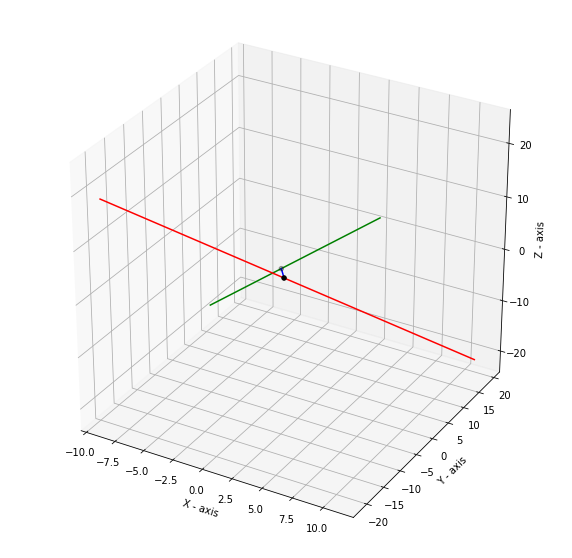
\includegraphics[width=\columnwidth]{./solutions/line_plane/80/assignment2.png}
    \caption{3-D plot for the skew lines and the shortest distance between them.}
    \label{skew_lines:solutions/line_plane/80}
\end{figure}

